\documentclass{beamer}

\usepackage{eurosym}
\usepackage{amsfonts}
\usepackage{amssymb}
\usepackage{amsmath}
%\usepackage{tipa}
\usepackage{array}
\usepackage{booktabs}
\usepackage{color}
\usepackage{epsfig,amssymb,latexsym,verbatim}
\usepackage{float}
\usepackage{graphicx}
\usepackage{graphicx, amssymb}
\usepackage{hyperref}
\usepackage{multicol}
\usepackage{multirow}
\usepackage{subfigure}
\usepackage{framed}
\usepackage{pifont}
\usepackage{colortbl}
\usepackage{comment}
\usepackage{booktabs}
\usepackage{ctex}

\newtheorem{lem}{引理}
\newtheorem{deff}{Definition}
\newtheorem{thm}{定理}
\newtheorem{proposition}{Proposition}
\newtheorem{coro}{推论}

\setcounter{MaxMatrixCols}{10}

\mode<presentation>

\def\cmd#1{\texttt{\color{red}\footnotesize $\backslash$#1}}
\def\env#1{\texttt{\color{blue}\footnotesize #1}}
\definecolor{deepblue}{rgb}{0,0,0.5}
\definecolor{deepred}{rgb}{0.6,0,0}
\definecolor{deepgreen}{rgb}{0,0.5,0}
\definecolor{halfgray}{gray}{0.55}
\definecolor{tsinghuapurple}{RGB}{175,0,26}
\definecolor{glassgrey}{rgb}{220,220,220}

% Set Colours
\mode<presentation> {
\usetheme{Madrid}
%\usecolortheme{beaver}
\setbeamercolor{structure}{bg=tsinghuapurple,fg=tsinghuapurple}
}
\author{李思雨}
\institute[SU]
{
\textbf{指导老师}: 张园园 \medskip \\ 
苏州大学数学科学学院
}

\DeclareMathOperator*{\argmax}{argmax}
\DeclareMathOperator*{\argmin}{argmin}
\DeclareMathOperator*{\BIC}{BIC}
\DeclareMathOperator*{\MSE}{MSE}

\begin{document}
 
\title[误差分布]{基于累积分布函数的非平稳空间序列统计推断}
\titlegraphic{
\includegraphics[width=2cm]{suda.jpeg}}
\date{2025/11/12}


\begin{frame}
\titlepage
\end{frame}

\begin{frame}{目录}
\begin{itemize}
\item 研究动机与思路 \medskip
\item 估计方法\medskip
\item 主要理论结果\medskip
\item 模拟研究 \medskip
\item 实际数据分析 \medskip
\item 总结
\end{itemize}
\end{frame}

\section{研究动机与思路}
\begin{frame}{研究动机与思路}
\begin{itemize}
\item \textbf{问题:} 
\begin{itemize}
\item 现有空间统计方法多适用规则网格区域, 难以处理\textbf{不规则图像域}(如带空洞或复杂边界).
\item 传统误差分布推断方法通常假设数据独立, 不适用于空间相关的图像数据.
\end{itemize}
\item \textbf{研究思路}
\begin{itemize}
\item 将不规则图像域划分为三角形网格, 构造局部多项式样条基函数(\cite{lai2013bivariate}, \cite{huq2023}), 用三角剖分上的二元样条(Bivariate Spline over Triangulations, BST)方法解决复杂边界和非矩形域的问题.
\item 在考虑数据空间相关性的前提下, 研究误差分布估计的Oracle有效性.(\cite{wang2020simultaneous}, \cite{wang2022oracle})
\item 基于估计的误差分布函数构造同时置信带(SCB), 量化不确定性.
(\cite{wang2020simultaneous})
\end{itemize}
\end{itemize}
\end{frame}


\section{估计方法}
\begin{frame}{估计方法：模型}
\begin{itemize}
    \item 我们考虑的模型是：
        \begin{equation}\label{model:nonparbiregression}
            Y_{\mathbf{i}} = g(X_{\mathbf{i}})+Z_{\mathbf{i}}, \mathbf{i}\in \mathcal{I}_n,
        \end{equation}
其中, $g(x):\mathbb{R}^2 \rightarrow \mathbb{R}$ 是光滑的二元非参函数,  $\{Z_{\mathbf{i}},\mathbf{i}\in\mathbb{Z}^2\}$ 是空间误差, 满足 $E(Z_{\mathbf{i}})=0$, 其概率密度函数为 $f(z)$，分布函数为 $F(z)=\int_{-\infty}^{z}f(u)du$.
    \item 数据量：$n = n_1*n_2$,
    \item 我们将索引集 $\mathcal{I}_n=\left\{\mathbf{i}_1,\cdots,\mathbf{i}_n\right\}$ 分为两个子集 $\mathcal{I}_{n'}=\left\{\mathbf{i}_{T_n},\cdots,\mathbf{i}_{n'T_n}\right\}$ and $ \mathcal{I}_{n''} = \mathcal{I}_{n}/\mathcal{I}_{n'}$, 其中 $T_{n}$是小于$n$的正整数, $n' = [n/T_{n}], n''=n-n'$.
\end{itemize}
\end{frame}




\begin{frame}{估计方法：BPST}
\begin{block}{数据划分}
\begin{itemize}
    \item 在数据集$\mathcal{I}_{n'}$上估计函数$g(\cdot)$;
    \item 基于数据集$\mathcal{I}_{n''}$计算残差$\hat{Z}_{\mathbf{i}'}$.
\end{itemize}
\end{block}

给定来自空间过程 $\{Y_{\mathbf{i}}\}$ 的观测样本$\mathbf{Y}=(Y_{\mathbf{i}''},\,\mathbf{i}''\in\mathcal{I}_{n''})^\top$， 
我们考虑以下最小二乘估计量：
\begin{equation}
  \hat{g}(\cdot)
  = \underset{s(\cdot)\in \mathbb{S}_{d}^{r}(\triangle)}{\mathrm{argmin}}
  \sum_{\mathbf{i}''\in\mathcal{I}_{n''}}\!
  \bigl\{Y_{\mathbf{i}''}-s(\boldsymbol{x}_{\mathbf{i}''})\bigr\}^2,
\end{equation}
其中，$\mathbb{S}_{d}^{r}(\triangle)$ 表示在三角剖分 $\triangle$ 上定义的次数为 $d$、光滑阶数为 $r$ 的样条函数空间。

\end{frame}

\begin{frame}{估计方法：KDE}
\begin{block}{Oracle核分布估计量}
对任意的oracle KDE
\begin{equation}\label{EQ:FN'hhat}
    \hat{F}_{n',h}(z) = \int_{-\infty}^{z}\hat{f}(u)du = n'^{-1}\sum_{\mathbf{i}'\in\mathcal{I}_{n'}}\int_{-\infty}^z K_h(u-\hat{Z}_{\mathbf{i}'})du,z\in\mathbb{R},
\end{equation}
其中残差$\hat{Z}_{\mathbf{i}'} = Y_{\mathbf{i}'} - \hat{g}(x_\mathbf{i'})$ 用于逼近真实误差 $Z_{\mathbf{i}'} = Y_{\mathbf{i}'} - g(x_\mathbf{i'})$, $\mathbf{i}'\in\mathcal{I}_{n'}$. 
\end{block}
\begin{block}{光滑同时置信带(SCB)的构造}
基于$\hat{F}_{n',h}(z)$可构造如下光滑同时置信带：
\begin{align} \label{SCB:FhatN'h}
    \left[\hat{F}_{n',h}(z)-\frac{L_{1-\alpha}}{\sqrt{n'}}, \hat{F}_{n',h}(z)+\frac{L_{1-\alpha}}{\sqrt{n'}}\right] \cap [0,1], z \in \mathbb{R},
\end{align}
\end{block}
\end{frame}

\begin{frame}{理论假设}
下面是本文用到的一些基础假设：

\begin{itemize}
\item[(A1)] 累积分布函数$F(\cdot) \in\mathcal{C}^{(1,1)}(\mathbb{R})$，其密度函数$f(\cdot)$ 满足 $\Vert f\Vert_{\infty}\leq C_f$（$C_f>0$为常数）.

\item[(A2)] 函数 $g(\cdot) \in \mathcal{W}^{\ell+1,\infty}(\Omega)$， 其中$\ell$为整数且$\ell\geq 1$.

\item[(A3)] 空间误差过程 $\{ Z_{\mathbf{i}} \}_{\mathbf{i} \in \mathcal{I}_n}$ 为空间$\alpha$-mixing过程且严格平稳.其有限矩$ M_{2+\delta} = \mathrm{E} |Z|^{2+\delta} < \infty $，$\delta > 0$。
此外，存在常数 $ C_\rho > 0,\rho \in (0,1) $，使得
\[
\alpha(k; i, j) \leq C_\rho i \rho^k, \quad \forall i, j, k \leq 1,
\]
其中，$\alpha(k; i, j)$ 表示强混合系数，常数 $C_\rho$和$\rho$ 都与 $i, j, k$ 无关。
\end{itemize}
\end{frame}

\begin{frame}{理论假设}
\begin{itemize}
\item[(A4)] 三角剖分 $\triangle$ 是 $\pi$ 拟均匀. 三角形数量满足 \( N = |\triangle|^{-2} = C n^\theta\)，其中常数 \( C > 0 \)，\( \theta \in \left[ 1/(\ell+2), 1 \right) \)。相邻点之间的间距 \[
T_n \sim |\triangle|^{-2} (\log n)^{a},
\]
其中 \( a > 0 \).
\label{Assumption:Delta}

\item[(A5)] 核函数 $K  \in\mathcal{C}^{(2,1)}(\mathbb{R})$为对称的概率密度函数, $K$ 及其导数 $K'$, $K''$的范围为$[-1,1].$ 

\item[(A6)]  带宽$h=h_n$满足$h=n'^{-t}c_n$, 其中$c_n+c_n^{-1}=o(\log ^{\tau} n)$ ($n \to \infty$, $\forall \tau > 0$), 且$t \in [1/4,1/3]$.
当$t=1/4$时, $c_n \to 0$.
\end{itemize}
\end{frame}

\section{主要理论结果}
\begin{frame}
\begin{proposition}[\cite{Yao2003ExponentialIF},\cite{bosq2012nonparametric}]
    在假设(A1)-(A4)成立的前提下, 当$n\to\infty$时,
    \[
\left\lVert \tilde{g} - g \right\rVert_{\infty} = \sup_{\boldsymbol{x} \in \Omega} \left| \tilde{g}(\boldsymbol{x}) - g(\boldsymbol{x}) \right| = \mathcal{O}_{a.s.} \left( |\triangle|^{\ell+1} \right),
\]
\end{proposition}

\begin{proposition}
[\cite{lai2007spline},\cite{yu2019estimation}]
  在假设(A1)-(A4)成立的前提下, 当 $n\to\infty$时,
  \[
\left\lVert \tilde{Z} \right\rVert_{\infty} = \sup_{\boldsymbol{x} \in \Omega} \left| \tilde{Z}(\boldsymbol{x}) \right| = \mathcal{O}_p \left( n''^{-1/2} |\triangle|^{-1} (\log n)^{1/2} \right),
\]  
\end{proposition}

\begin{proposition}
    在假设(A1)-(A4)成立的前提下, 当 $n\to\infty$时,
   \[
\max_{\mathbf{i}' \in \mathcal{I}_{n'}} \left\lVert Z_{\mathbf{i}'} - \hat{Z}_{\mathbf{i}'} \right\rVert 
\le \left\lVert \hat{g} - g \right\rVert_{\infty}
= \mathcal{O}_p \left( |\triangle|^{\ell+1} + n''^{-1/2} |\triangle|^{-1} (\log n)^{1/2} \right).
\]
\end{proposition}
\end{frame}


\begin{frame}{定理\uppercase\expandafter{\romannumeral 1}}
\begin{thm} \label{THM:FhatFtilde}
在假设(A1)-(A6)成立的前提下, oracle估计量$\hat{F}_{n',h}(\cdot)$ 渐近等价于infeasible估计量$\tilde{F}_{n',h}(\cdot)$, 即当$n\to\infty$时，
\begin{align*}
    D\left(\hat{F}_{n',h}, \tilde{F}_{n',h}\right) = \left\Vert\hat{F}_{n',h} - \tilde{F}_{n',h}\right\Vert_{\infty} = {\scriptstyle{\mathcal{O}}}_{p}\left(n'^{-1/2}\right).
\end{align*}
\end{thm}
根据(\cite{fazekas2006asymptotic})的研究, 当$n\to\infty$时, \[
n'^{1/2}\left(F_{n'}(\cdot) - F(\cdot)\right) \overset{D}{\rightarrow} \mathcal{B}(F(\cdot)),
\]
其中$\mathcal{B}(\cdot)$ 是标准布朗桥.  
结合上述定理\ref{THM:FhatFtilde}以及(\cite{wang2013smooth})的结果$\left\Vert\tilde{F}_{N',h} - F_{N'}\right\Vert_{\infty} = {\scriptstyle{\mathcal{O}}}_{p}\left(N'^{-1/2}\right)$, 可得$\left\Vert\hat{F}_{N',h} - F_{N'}\right\Vert_{\infty}={\scriptstyle{\mathcal{O}}}_{p}\left(N'^{-1/2}\right)$. 因此可推出如下结论：
\end{frame}

\begin{frame}{置信区间}
    \begin{coro}
  在定理\ref{THM:FhatFtilde}的假设条件下, 当 $n \to \infty$时,
    \begin{align*}
           N'^{1/2}\left(\hat{F}_{N',h}(\cdot)-F(\cdot)\right)\overset{d}{\rightarrow} W(\cdot),  
    \end{align*}
特别地，
\begin{align*}
    \sqrt{N'\Gamma^{-1}}\left(\hat{F}_{N',h}(\cdot)-F(\cdot)\right)\overset{d}{\rightarrow} N(0,1),\forall z \in \mathbb{R}.
\end{align*}
因此，当$\alpha \in (0,1)$时,
\begin{align*}
    \lim_{N' \to \infty}P\left\{F(z) \in \hat{F}_{N',h}(z) \pm L_{1-\alpha}/\sqrt{N'}, z\in  \mathbb{R}\right\}=1-\alpha,
\end{align*}
 为$F(z)$的光滑SCB，定义在(\ref{SCB:FhatN'h}).
\end{coro}
\end{frame}


\section{模拟研究}
\begin{frame}{模拟研究}
\begin{itemize}
    \item 我们分别在规则区域和不规则区域(shape)上计算了误差分布的估计量最大偏差.

    \item 数据生成的样本大小为$N=100*100, 100*200, 180*180, 200*200$.

    \item 数据由以下模型生成：
        $$Y_{\mathbf{i}} = g(x_1,x_2)+Z_{\mathbf{i}},\mathbf{1}\leq \mathbf{i}\leq \mathbf{n},$$
其中，回归函数为： $g(x_1,x_2) = sin(\pi x_1)+exp(-x_2^2)$.
\end{itemize}
\end{frame}




\begin{frame}{模拟研究}
\begin{table}[!htb]
\caption{ 规则区域上三种估计量平均最大偏差的对比}
\begin{center}
\begin {tabular}{cccc}
    \hline
    Deviations & Sample Size & N$(0,1)$ & t$(10)$ \\
    \hline
    \multirow{4}{*}{$\bar{D}(\hat{F}_{N',h},F)$} 
        & $n_1=100, n_2=100$  & $0.0340$ & $0.0345$ \\
        & $n_1=200, n_2=100$  & $0.0294$ & $0.0300$ \\
        & $n_1=180, n_2=180$  & $0.0233$ & $0.0245$ \\
        & $n_1=200, n_2=200$  & $0.0209$ & $0.0209$ \\
    \hline
    \multirow{4}{*}{$\bar{D}(\hat{F}_{N'},F)$} 
        & $n_1=100, n_2=100$  & $0.0340$ & $0.0350$ \\
        & $n_1=200, n_2=100$  & $0.0294$ & $0.0302$ \\
        & $n_1=180, n_2=180$  & $0.0247$ & $0.0265$ \\
        & $n_1=200, n_2=200$  & $0.0225$ & $0.0225$ \\ 
    \hline
    \multirow{4}{*}{$\bar{D}(\tilde{F}_{N'},F)$} 
        & $n_1=100, n_2=100$  & $0.0333$ & $0.0340$ \\
        & $n_1=200, n_2=100$  & $0.0287$ & $0.0292$ \\
        & $n_1=180, n_2=180$  & $0.0219$ & $0.0220$ \\
        & $n_1=200, n_2=200$  & $0.0199$ & $0.0204$ \\
    \hline
\end{tabular}
\end{center}
\end{table}
\end{frame}

\begin{frame}{模拟研究}
\vspace{-0.1cm}
\begin{figure}
\vspace{-0.5cm}
\caption{规则区域上$D\left( \hat{F}_{N^{\prime },h},F\right) $ 的箱线图 }
\centering
    \begin{minipage}[t]{\linewidth}
        \centering
        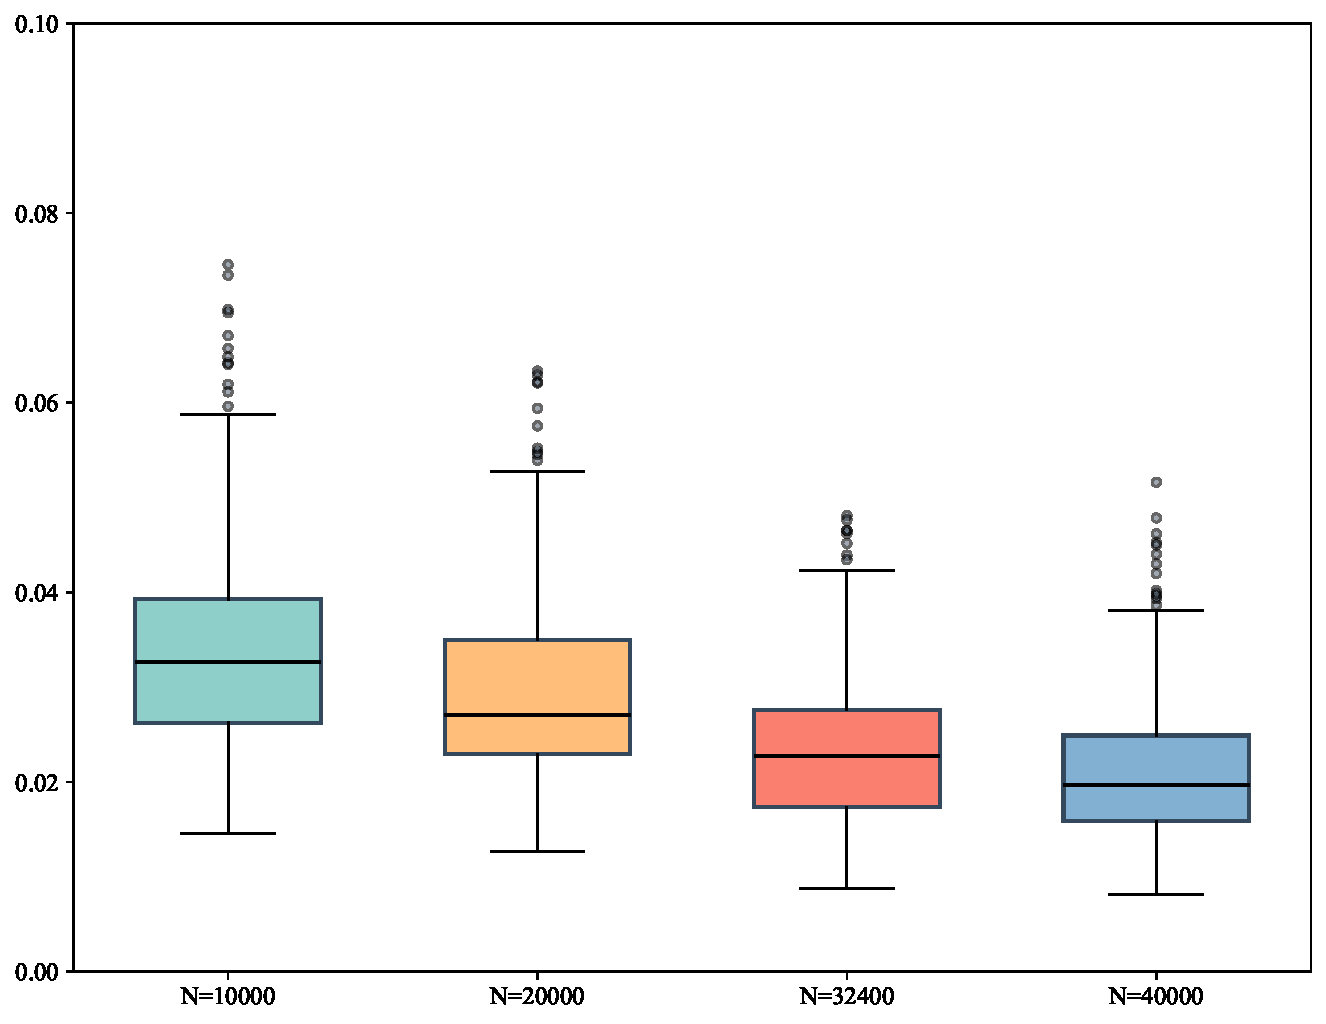
\includegraphics[width=0.7\linewidth]{boxplot_regular_normal.pdf}
    \end{minipage}
\end{figure}
\end{frame}


\begin{frame}{模拟研究}
\begin{table}[!htb]
\caption{ 不规则区域shape上三种估计量平均最大偏差的对比}
\begin{center}
\begin {tabular}{cccc}
    \hline
    Deviations & Sample Size & N$(0,1)$ & t$(10)$ \\
    \hline
    \multirow{4}{*}{$\bar{D}(\hat{F}_{N',h},F)$} 
        & $n_1=100, n_2=100$   & 0.0475 & 0.0476 \\
        & $n_1=200, n_2=100$   & 0.0413 & 0.0422 \\
        & $n_1=180, n_2=180$   & 0.0342 & 0.0340 \\
        & $n_1=200, n_2=200$   & 0.0296 & 0.0304 \\
    \hline
    \multirow{4}{*}{$\bar{D}(\hat{F}_{N'},F)$} 
        & $n_1=100, n_2=100$   & 0.0479 & 0.0483 \\
        & $n_1=200, n_2=100$   & 0.0417 & 0.0428 \\
        & $n_1=180, n_2=180$   & 0.0370 & 0.0376 \\
        & $n_1=200, n_2=200$   & 0.0311 & 0.0312 \\
    \hline
    \multirow{4}{*}{$\bar{D}(\tilde{F}_{N'},F)$} 
        & $n_1=100, n_2=100$   & 0.0468 & 0.0479 \\
        & $n_1=200, n_2=100$   & 0.0414 & 0.0409 \\
        & $n_1=180, n_2=180$   & 0.0331 & 0.0316 \\
        & $n_1=200, n_2=200$   & 0.0292 & 0.0310 \\
    \hline
\end{tabular}
\end{center}
\end{table}
\end{frame}

\begin{frame}{模拟研究}
\vspace{-0.1cm}
\begin{figure}
\vspace{-0.5cm}
\caption{ 不规则区域shape上$D\left( \hat{F}_{N^{\prime },h},F\right) $ 的箱线图}
\centering
        \begin{minipage}[t]{\linewidth}
        \centering
        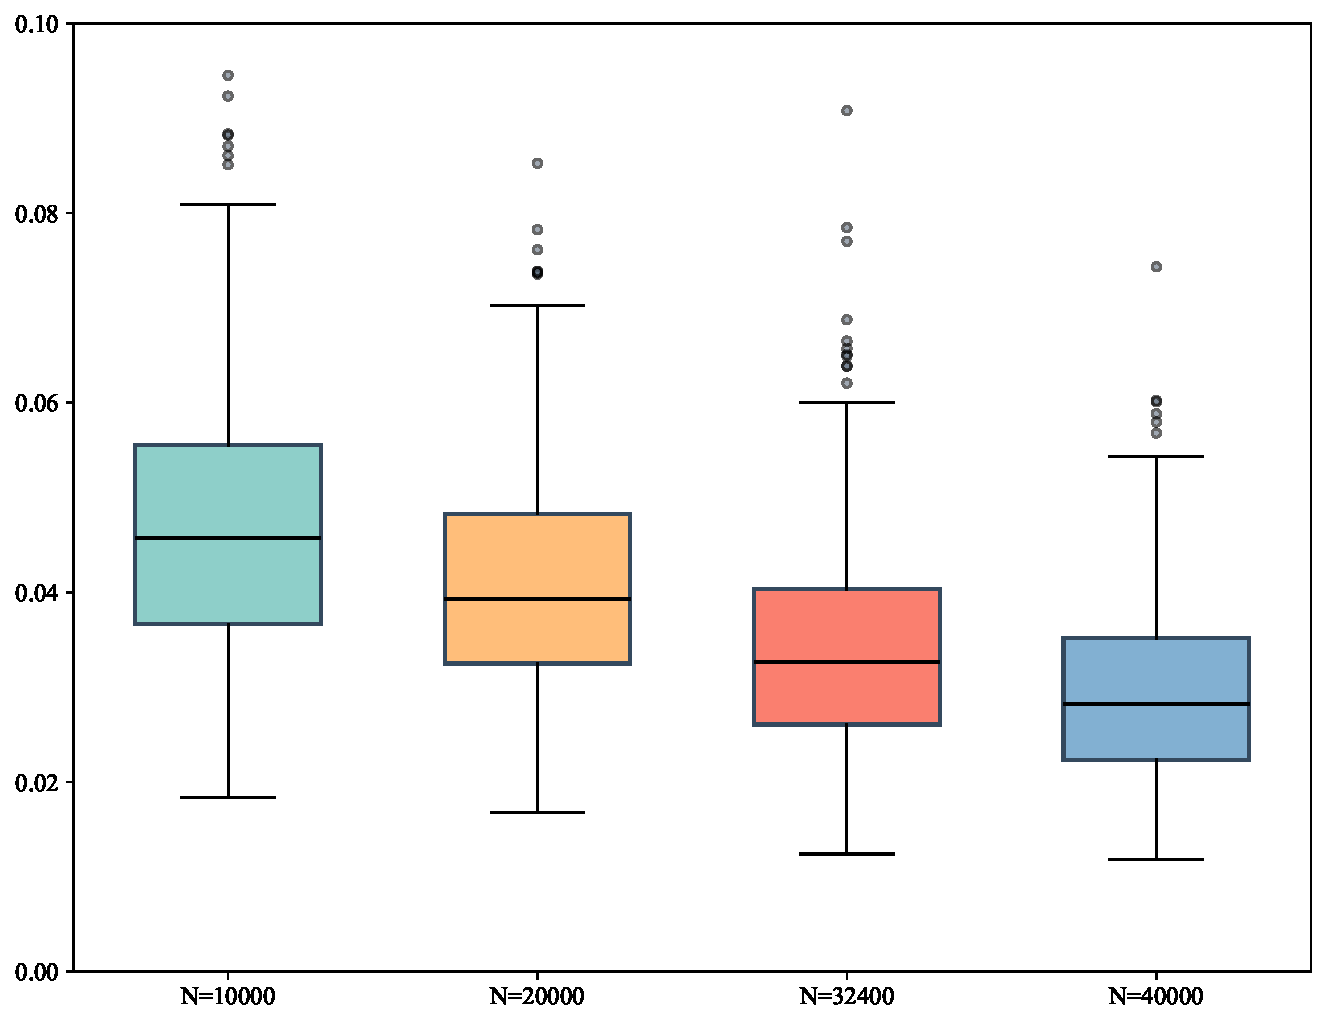
\includegraphics[width=0.7\linewidth]{boxplot_irregular_normal.pdf}
    \end{minipage}
\end{figure}
\end{frame}

\section{实际数据分析}
\begin{frame}{实际数据分析}
\begin{itemize}
    \item 真实数据选取我国东海和南海的海表温度数据. \cite{huq2023}, \cite{cai2024global}.
        \begin{itemize}
            \item 东海经纬度范围：$22.5^{\circ}$N - $34.5^{\circ}$N和$118^{\circ}$E - $128^{\circ}$E.
            \item 南海经纬度范围：$3^{\circ}$N - $25^{\circ}$N和$105^{\circ}$E - $125^{\circ}$E.
        \end{itemize}
    \item 数据来源：国家海洋科学数据中心\\
    \url{https://mds.nmdis.org.cn/}.
\end{itemize}
\end{frame}



\section{总结}
\begin{frame}{总结}
\begin{itemize}
    \item 在假设条件下，证明了二维不规则域上非参回归误差分布估计的渐近理论, oracle效率为${\scriptstyle{\mathcal{O}}}_{p}\left(N'^{-1/2}\right)$.
    \item 构建了适用于复杂区域的误差分布同时置信带(SCB).
\end{itemize}
\end{frame}


\begin{frame}{References}
\fontsize{7pt}{2pt}
\bibliography{sn-bibliography}
\begin{thebibliography}{20}

\bibitem[Hu(2023+)]{huq2023}
Hu Qirui and Li Jie (2023+). Statistical inference for mean function of longitudinal imaging data over complicated domains. Statistica Sinica 34, 955-982.
\bibitem[Cai(2024)]{cai2024global}
Cai, Leheng and Hu, Qirui (2024). Global inference and test for eigensystems of imaging data over complicated domains. Journal of Computational and Graphical Statistics, 1-17.
\bibitem[Wang(2022)]{wang2022oracle}
Wang, Jiangyan and Gu, Lijie and Yang, Lijian (2022). Oracle-efficient estimation for functional data error distribution with simultaneous confidence band. Computational Statistics \& Data Analysi 167, 107363.
\bibitem[Lai(2013)]{lai2013bivariate}
Lai, Ming-Jun and Wang, Li (2013). Bivariate penalized splines for regression. Statistica Sinica 23, 1399-1417.
\bibitem[Wang(2020)]{wang2020simultaneous}
Wang, Yueying and Wang, Guannan and Wang, Li and Ogden, R Todd (2020). Simultaneous confidence corridors for mean functions in functional data analysis of imaging data. Biometrics 76(2), 427-437.
\bibitem[Lai(2007)]{lai2007spline}
Lai, Ming-Jun and Schumaker, Larry L (2007). Spline Functions on Triangulations. Cambridge University Press.
\bibitem[Yu(2019)]{yu2019estimation}
Yu, Shan and Wang, Guannan and Wang, Li and Liu, Chenhui and Yang, Lijian (2019). Estimation and inference for generalized geoadditive models. Journal of the American Statistical Association 115, 761-774.
\bibitem[Bosq(2012)]{bosq2012nonparametric}
Bosq, Denis (2012). Nonparametric Statistics for Stochastic Processes: Estimation and Prediction. Springer Science \& Business Media.
\bibitem[Yao(2003)]{Yao2003ExponentialIF}
Yao, Qiwei (2003). Exponential inequalities for spatial processes and uniform convergence rates for density estimation. Development Of Modern Statistics And Related Topics, 118-128.
\bibitem[Fazekas(2006)]{fazekas2006asymptotic}
Fazekas, Istv{\'a}n and Chuprunov, Alexey (2006). Asymptotic normality of kernel type density estimators for random fields. Statistical inference for stochastic processes 9, 161-178.
\bibitem[Wang(2013)]{wang2013smooth}
Wang, Jiangyan and Cheng, Fuxia and Yang, Lijian (2013). Smooth simultaneous confidence bands for cumulative distribution functions. Journal of Nonparametric Statistics, 395-407.
\end{thebibliography}
\end{frame}

\begin{frame}
\begin{center}
\Huge{ 谢谢大家 !}
\end{center}
\end{frame}

\end{document}
